\documentclass[a4paper,12pt]{article} 
\usepackage{kotex} 
\usepackage[figuresright]{rotating} 
\usepackage{fancyhdr}
\usepackage{indentfirst}
\usepackage{relsize}
\usepackage{miama}
\usepackage[T1]{fontenc}
\usepackage[inline]{enumitem}
\usepackage{multicol}
\usepackage{amsmath}	% \text
\usepackage{amssymb}

\usepackage{booktabs}

\usepackage{fontspec}
\setmainfont{Times New Roman}

\usepackage{hyperref} 	% To make tableofcontents hyperlinkable
\hypersetup{
    colorlinks=true,
	linktoc=all,
	linkcolor=black
}



\usepackage{listingsutf8}		%  Listing with UTF-8!
\usepackage[dvipsnames]{xcolor}

\lstset{
	language         = python,
	basicstyle       = \ttfamily\relsize{-1},
    keywordstyle     = \color{blue},%\bfseries,
    identifierstyle  = \bfseries,
    commentstyle     = \color{olive},
    moredelim        = [s][\color{ForestGreen}]{/**}{*/},	% For doxygen-style comments
    stringstyle      = \color{magenta},
    frame            = lines,
    showstringspaces = false,
    columns          = flexible,
	breaklines		 = true,
	tabsize          = 4,
	numbers          = left,
	numbersep        = 4pt,
	numberstyle      = \tiny\color{gray},
	mathescape       = true
}


%\pagestyle{fancy}
%\lhead{}
%\rhead{}

\begin{document} 
%1페이지
\title{CS560: Systems for machine Learning\\\large Project 1 Report}
\author{Jehoon Park\\Junoh Moon\\\\Korea Advanced Institute of Science and Technology}
\date{\today}

%1페이지 로고
\begin{figure}[!b]
	\centering
	
\includegraphics[width=0.7\textwidth]{./kaist_emblem2.eps}
	\label{figure:school_logo}
\end{figure}

\maketitle
\thispagestyle{empty} %Ignore page number of first page
\newpage
%page 2

\section{Overview}
In the first assignment, we were required to build a \emph{Tiny YOLOv2} model using tensorflow and detect objects with pretrained weights. The code required to detect objects works as follows. First, the video clip is splitted into frames. Each frame is resized into $416 \times 416$ for the purpose of the model's input. The model infers `bounding boxes', which are sets of the class of objects and their locations, for each frame. This procedure includes non-max-suppression. After inferred, the bounding boxes are resized to the original clip resolution and drawn on the original frame.
For each device, CPU and GPU, the inference time and end-to-end time were measured; compared to CPU, GPU performed 1.84 times faster on end-to-end time due to 3.88 times faster inference time.

\section{Implementation}


\subsection{Building model}

To detect objects, a \emph{YOLO\_V2\_TINY} instance was created by invoking \lstinline{__init__} method itself. 
While invoked, the method generated the model by stacking composite layers, configuring some GPU options, creating its own session and graph, and so on. 
Each composite layer consists of 1--5 base layers: \lstinline{tf.nn.conv2d}, \lstinline{tf.nn.bias_add}, \lstinline{tf.nn.batch_normalization}, \lstinline{tf.maximum}, and \lstinline{tf.nn.max_pool2d}.
In addition, some base layers --- \lstinline{conv2d}, and \lstinline{bias_add}, and \lstinline{batch_normalization} --- were initialized with pretrained weight parameters by passing the parameter which is wrapped into \lstinline{tf.Variable};
‘kernel’ was used for \lstinline{conv2d}; 
‘bias’ was used for \lstinline{bias_add};
finally ‘moving\_variance’, ‘gamma’, and ‘moving\_mean’ were used for \lstinline{batch_normalization}. Furthermore, \lstinline{tf.maximum} was used for implementing leakyRelu layer and \lstinline{max_pool2d} layer was set by a $(2 \times 2)$ kernel and a $(2 \times 2)$ stride except the last \lstinline{max_pool2d}, which was set by $(1 \times 1)$ stride. Therefore, the \emph{Tiny YOLOv2} model was generated as Figure \ref{figure:graph}.
Although the main logic was completed, some implementation details still remained. For the sake of preventing memory error in GPU mode, \lstinline{per_process_gpu_memory_fraction} configuration was added.

\begin{figure}
	\centering
	
\includegraphics[width=\textwidth]{./model}
	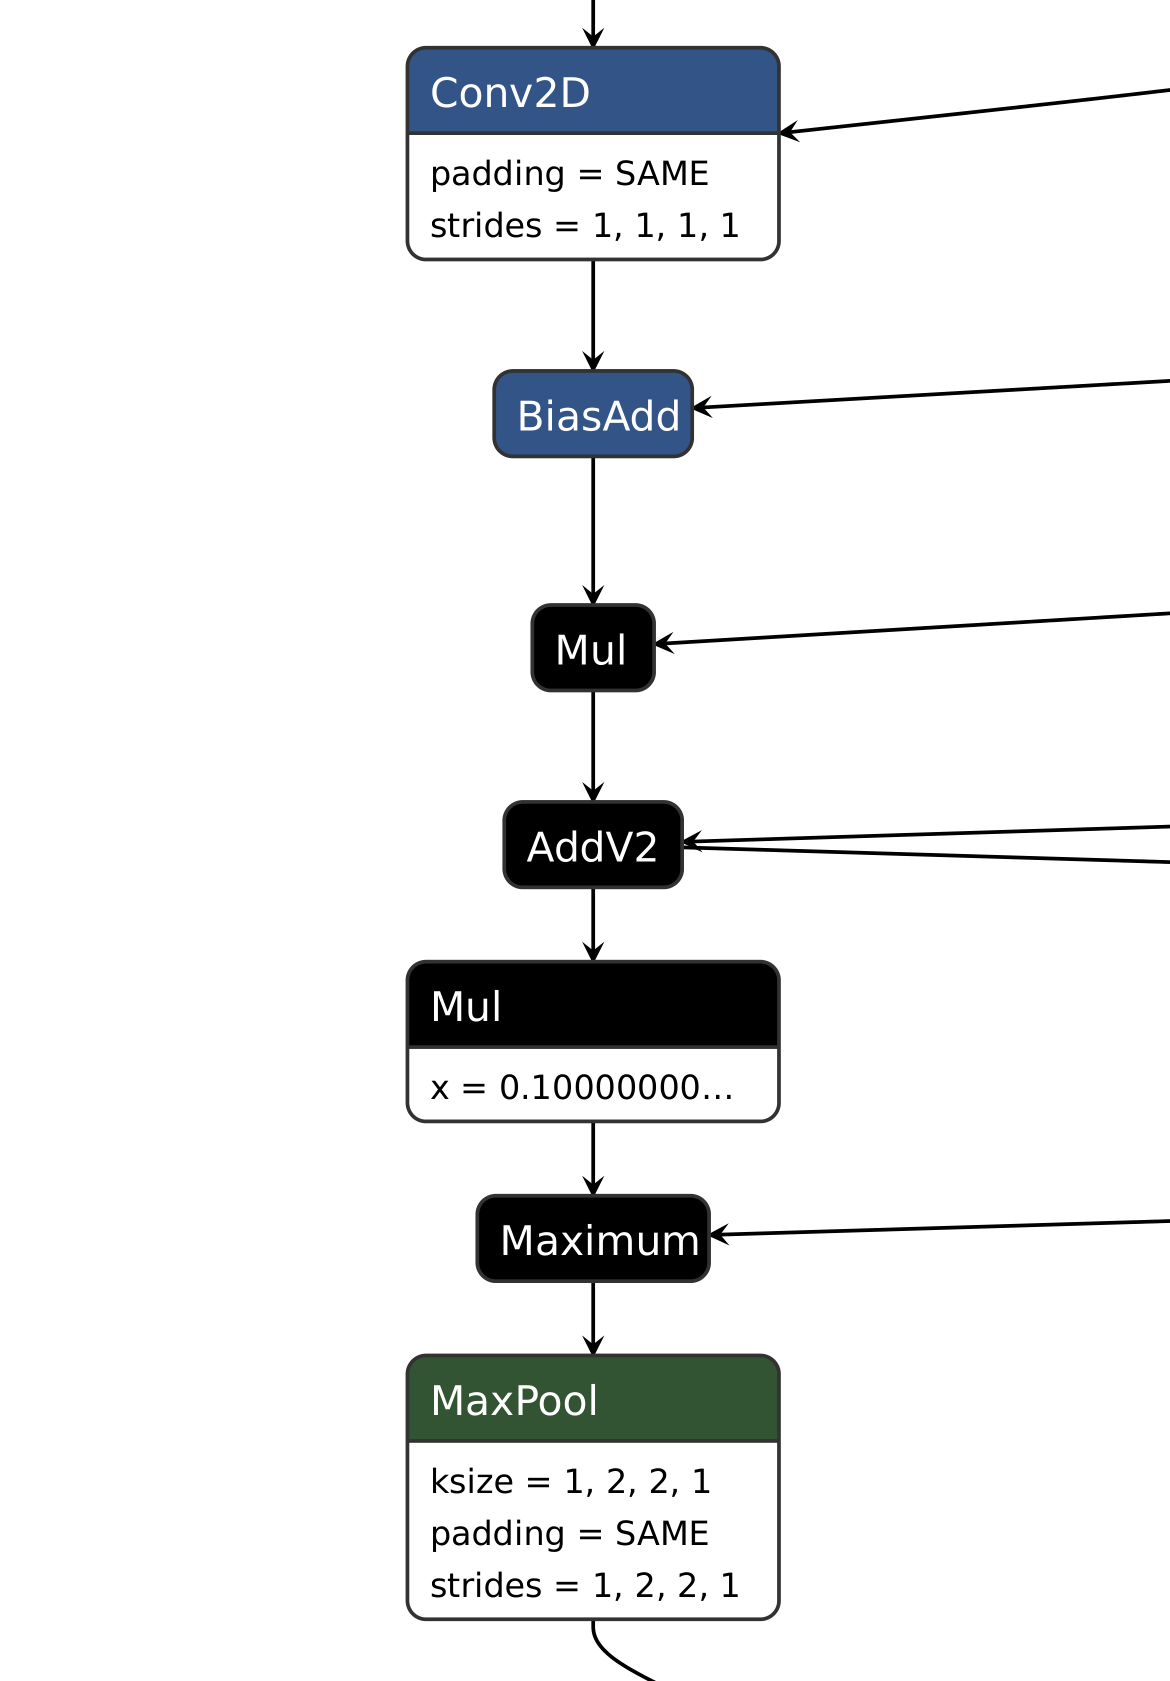
\includegraphics[height=0.5\textheight]{./model_crop3}
	\caption{The above figure is the entire graph generated and restored by Tensorflow. 
	The other is the cropped figure of the above since the whole graph is too verbose to recognize how it is modeled.
	Therfore, we cropped for focusing one main-composite-layer which consists of \lstinline{conv2d}, \lstinline{batch_normalization}, \lstinline{leakyRelu}, and so on.
	}
	\label{figure:graph}
\end{figure}


\subsection{Video processing}
Since input data was given in video clips, we had to split into a set of images. For the purpose of video processing, openCV was chosen. By using VideoCapture and VideoWriter in openCV, we could split a clip into frames and merge into a clip. While initiated, a VideoWriter instance had to keep the original clip’s information: FPS, width, height, and fourcc (codec). To keep them the same, \lstinline{VideoCapture.get} method was invoked. However, fourcc value couldn’t be equal to the original on account of the lack of supporting codecs in the OS, so it was hard-coded into “mp4v”.
Furthermore, both two instances must be verified that clips are opened well. The instances were designed to raise an exception unless the video clip was opened correctly.

\subsection{Detection}
After boilerplate codes were executed, the main loop started.
 First, each frame was resized into $416 \times 416$, since the input shape of the \lstinline{YOLO_V2_TINY} instance is $(\textit{batch}, 416, 416, 3)$.
 After being resized, tensors were inferred by the instance.
 The tensors are a set of bounding boxes, whereas they were not yet enough to represent objects in the frame because there were bounding boxes with a low confidence score than threshold, and the objects in the frame were pointed by too many bounding boxes.

Thus, two steps were processed in \emph{YOLO\_V2\_TINY}.
postprossing’ method; the first step is filtering bounding boxes whose score is lower than threshold; the second step is ‘non-max-suppression’, which only lefts the best bounding box and remove others per object.
Finally, each object was labelled on the frame through the given post-processed bounding boxes. 

\section{Evaluation}
% Please add the following required packages to your document preamble:
\begin{table}[h!]
	\centering
	\resizebox{\textwidth}{!}{%
		\begin{tabular}{@{}lccccc@{}}
			\toprule
			& Total (sec) & Average end-to-end (sec/frame) & Average end-to-end (FPS) & Average inference (sec/frame) & Average inference (FPS) \\ \midrule
			CPU & 44.0003 & 0.0598 & 10.2976 & 0.0971 & 16.7252 \\
			GPU & 23.8910 & 0.0527 & 18.9753 & 0.0154 & 64.9773 \\ \bottomrule
		\end{tabular}%
	}
	\caption{This results are averages of 100 indivisual experiments.}
	\label{tab:eval}
\end{table}
The total time is the time of processing the whole video clip. End-to-end time includes preprocessing input frame, inference, post processing, and writing the result clip.
It was shown that the GPU performed the whole process faster about 1.84 times  than the CPU\@.
 This result was due to the faster inference time of GPU\@. During the inference, the \emph{Tiny YOLOv2} performs convolution layers, which require nested loops computation.
GPU’s highly parallel architecture can handle this kind of calculations better than CPU, so the inference time was decreased significantly about 3.88 times. 
Since the inference part was about 60\% of total computation, the total execution time was improved about 1.84 times.

\section{Discussion}
The result was shown that the pre and post processing time were the same on both devices. These parts were computed in sequential only on CPU\@. 
However, there is a triple-nested loop in the post processing part, so it looks possible that if we use GPU for these computations, the execution time will be faster.

% Please add the following required packages to your document preamble:
% \usepackage{booktabs}
\begin{table}[!h]
	\centering
	\begin{tabular}{@{}cccc@{}}
		\toprule
		 & \multicolumn{3}{c}{Inference time (sec)} \\ \cmidrule(l){2-4} 
		  & 1st & 2nd & 3rd \\ \midrule
		  GPU & 1.252 & 0.103 & 0.011 \\ \midrule
		  CPU & 0.153 & 0.078 & 0.047 \\ \bottomrule
	\end{tabular}
	\caption{The first three inference times on GPU and CPU.}
	\label{tab:each_inference}
\end{table}

Interesting result was shown at the beginning of the ‘session.run’. On CPU, it took 0.153 seconds to inference the first frame, while the average time was 0.060.
Moreover, on the GPU, it took 1.252 seconds for the inference first frame and 0.103 for the second, while the average was 0.015.
These were because at the beginning, the tensorflow performed initializations. Also, the significant slow first run time of GPU was because the tensorflow used cuDNN’s autotune feature for convolution layers to compute them faster.  


\subsection{Code}
\subsubsection{\_\_init\_\_.py}
\lstinputlisting{../__init__.py}
\subsubsection{yolov2tiny.py}
\lstinputlisting{../yolov2tiny.py}

\end{document}

